\documentclass[a4paper, 12pt]{article}

\usepackage{prelab}

\usepackage{graphicx}
\usepackage{pgfplots}
\usepackage{pgfplotstable}
\usepackage{titlesec}
\usepackage{listings}

\pgfplotsset{width=12cm, compat=1.18}

\begin{document}

\prefixlab{1}{Введение в паралеллельные вычисления. Технолония OpenMP}

\section{Анализ алгоритма}

\subsection{Принцип работы}

Алгоритм является поиском элемента в массиве.
Программа:
\begin{enumerate}
    \item Выделяет память под массив, инициализирует генератор случайных значений;
    \item Заполняет массив случайными числами;
    \item Ищет элемент с определенными настройками \textit{OpenMP}.
\end{enumerate}

Результатом поиска является индекс элемента в массиве.
Поиск осуществляется последовательно.

Временная сложность алгоритма $O(n)$, где $n$ -- число элементов в массиве.


Блок-схема алгоритма выглядит следующим образом:\\
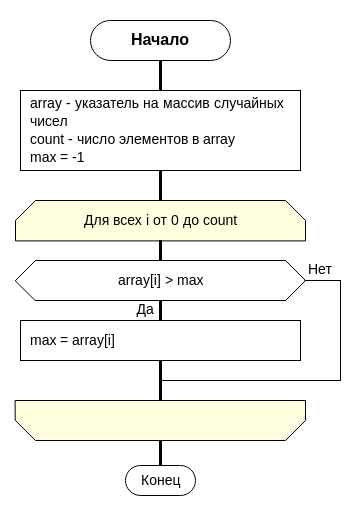
\includegraphics[scale=0.6]{res/flowchart.png}

\subsection{Параллелизация}

Аналогично предыдущей лабораторной работе алгоритм можно параллелизовать, распределив итерации между потоками.
Единственное существенное отличие -- если элемент был встречен, то необходимо в тот же момент выйти из цикла.

Рассмотрим задаваемые опции параллелизации:
\begin{itemize}
    \item \textit{num\_threads} - число используемых потоков;
    \item \textit{shared(array, N, index, target)} - общая для всех потоков память (переменные). Сюда включены массив, его размер, индекс искомого элемента (для сохранения результата) и искомое значение соответсвенно;
    \item \textit{default(none)} - локальность всех переменных, не указанных в \textit{shared}.
\end{itemize}

Для преждевременного прерывания поискового цикла (аналог \textit{break}) будет использоваться \textit{omp cancel for}.
Эта директива прервет все потоки как только искомый элемент будет найден.
Для работы директивы \textit{omp cancel for} может потребоваться установка переменной окружения \textit{OMP\_CANCELLATION=true}.

Также так как используется общая переменная \textit{index}, в операциях с ней следует использовать \textit{omp critical}.

\section{Экспериментальные данные}

На каждое число потоков отводилось 20 запусков.

\subsection{Время выполнения}

Для начала я решил взглянуть не только на среднюю скорость выполнения, но и на крайние варианты:

\vspace{0.5cm}

\begin{tikzpicture}
    \begin{axis}[
        xlabel={Число потоков},
        ylabel={Время (мс)},
        legend pos=north east,
    ]
    \addplot table [x index = 0, y index = 1, col sep=comma] {data/base.csv};
    \addplot table [x index = 0, y index = 2, col sep=comma] {data/base.csv};
    \addplot table [x index = 0, y index = 3, col sep=comma] {data/base.csv};
    \legend{Худшее время, Лучшее время, Среднее время}
    \end{axis}
\end{tikzpicture}

\vspace{0.5cm}

Крайне заметно, что многопоточная программа работает куда быстрее её конкурентов.
Единственным исключением является запуск при 2-x потоках.

Аналогично первой лабораторной рассмотрим теперь данные с оптимизацией:

\vspace{0.5cm}

\begin{tikzpicture}
    \begin{axis}[
        xlabel={Число потоков},
        ylabel={Время (мс)},
        legend pos=north east,
    ]
    \addplot table [x index = 0, y index = 1, col sep=comma] {data/opt.csv};
    \addplot table [x index = 0, y index = 2, col sep=comma] {data/opt.csv};
    \addplot table [x index = 0, y index = 3, col sep=comma] {data/opt.csv};
    \legend{Худшее время, Лучшее время, Среднее время}
    \end{axis}
\end{tikzpicture}

\vspace{0.5cm}

Как видно на графике выше, повышение числа потоков уменьшает среднее время исполнения.

\subsection{Прирост производительности}

В целом с увеличением числа потоков производительность растет.
Рассмотрим ускорение многопоточной программы относительно однопоточной.
Для не оптимизированной сборки:

\vspace{0.5cm}

\begin{tikzpicture}
    \begin{axis}[
        xlabel={Число потоков},
        ylabel={Прирост (\%)},
        ybar interval=0.7,
    ]
    \addplot table [x index = 0, y index = 1, col sep=comma] {data/cmp_base.csv};
    \end{axis}
\end{tikzpicture}

\vspace{0.5cm}

Для оптимизированной сборки:

\vspace{0.5cm}

\begin{tikzpicture}
    \begin{axis}[
        xlabel={Число потоков},
        ylabel={Прирост (\%)},
        ybar interval=0.7,
    ]
    \addplot table [x index = 0, y index = 1, col sep=comma] {data/cmp_opt.csv};
    \end{axis}
\end{tikzpicture}

\vspace{0.5cm}


\section{Заключение}

В данной работе было исследовано ускорение, получаемое при использовании нескольких потоков в задании о поиске максимума.
Была усовершенствована предоставленная программа и собранны данные.
Так же был написан скрипт, подсчитывающий прирост производительности относительно одного потока.
Оформлен отчет.

В ходе работы было выяснено, что в применение нескольких потоков крайне положительно влияет на итоговую производительность.
Из 30 многопоточных сборок только одна была медленнее однопоточной.
При этом наблюдался прирост вплоть до 3х раз.

\appendix

\titleformat{\section}[display]
  {\normalfont\Large\bfseries}
  {\centering Приложение\ \thesection\\}
  {0pt}{\Large\centering}
\renewcommand{\thesection}{\Asbuk{section}}

\section{Использованные программные коды}

Для проверки версии \textit{OpenMP} использовался следующий код:
\lstinputlisting[language=C, basicstyle=\small]{code/omp_ver.c}
\vspace{0.5cm}

Код, использовавшийся для проверки функциональности \textit{MPI}
\lstinputlisting[language=C, basicstyle=\tiny]{code/original.c}
\vspace{0.5cm}

Для измерения времени исполнения программы с использованием \textit{OpenMP} использовался следующий код(выводит \textit{csv} в стандартный вывод):
\lstinputlisting[language=C, basicstyle=\tiny]{code/omp_main.c}
\vspace{0.5cm}

Для измерения времени исполнения программы с использованием \textit{MPI} использовался следующий код(выводит \textit{csv} в стандартный вывод):
\lstinputlisting[language=C, basicstyle=\tiny]{code/omp_main.c}
\vspace{0.5cm}

А так же для этой цели использовался скрипт:
\lstinputlisting[language=Python, basicstyle=\tiny]{code/runmpi.py}
\vspace{0.5cm}

\section{Таблицы c практическими результатами}

\textit{OpenMP}:

\vspace{0.3cm}

\pgfplotstabletypeset[
 col sep=comma,
 columns={Threads,Worst (ms),Best (ms),Avg (ms)},
]{data/omp.csv}

\vspace{0.5cm}

\textit{MPI}:

\vspace{0.3cm}

\pgfplotstabletypeset[
 col sep=comma,
 columns={Threads,Worst (ms),Best (ms),Avg (ms)},
]{data/mpi.csv}

\vspace{0.5cm}


\end{document}
